%% LaTeX 图表代码片段 - HW-1 学术论文
%% 自动生成于 generate_all_figures.py

% ============================================================================
% 图1: 版本演化时间线
% ============================================================================
\begin{figure}[htbp]
  \centering
  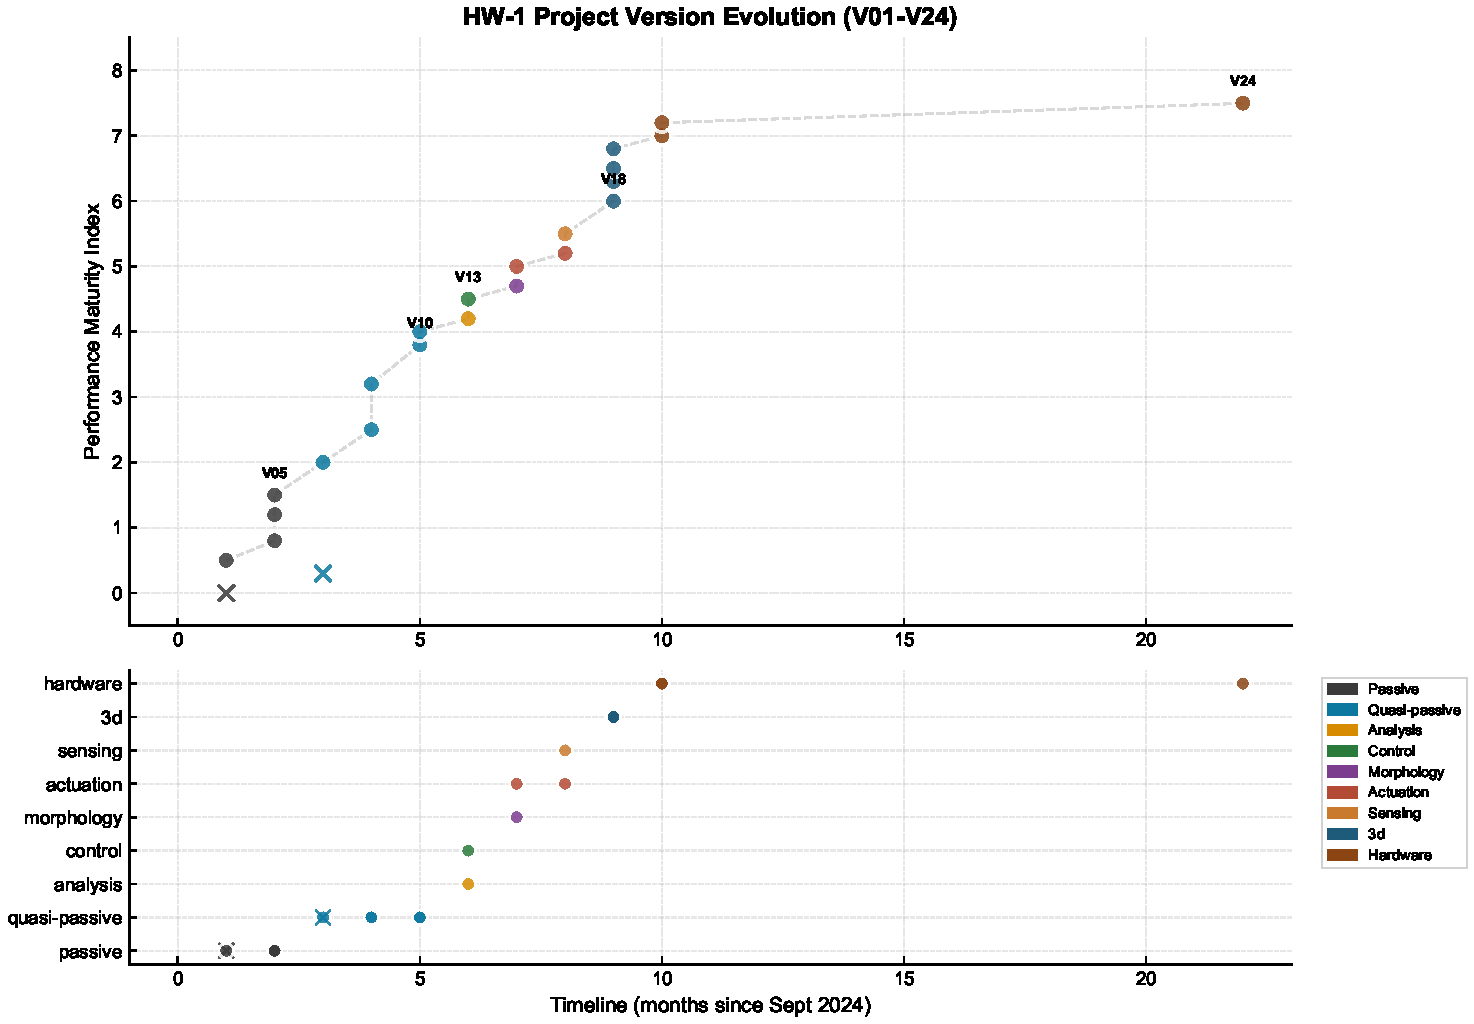
\includegraphics[width=\textwidth]{paper_figures/output/fig1_version_evolution.pdf}
  \caption{版本演化时间线：V01（指南针步态）至V25（实地行走）的开发进程。
  上图显示性能成熟度指数演进，下图展示各版本类别分布。
  关键里程碑：V05（纯被动极限环证明）、V10（足踝滚动）、V13.7（摩擦补偿FSM）、
  V17（状态估计闭环）、V22（硬件设计）。}
  \label{fig:version_evolution}
\end{figure}

% ============================================================================
% 图2: 参数空间稳定域（V13切片C）
% ============================================================================
\begin{figure}[htbp]
  \centering
  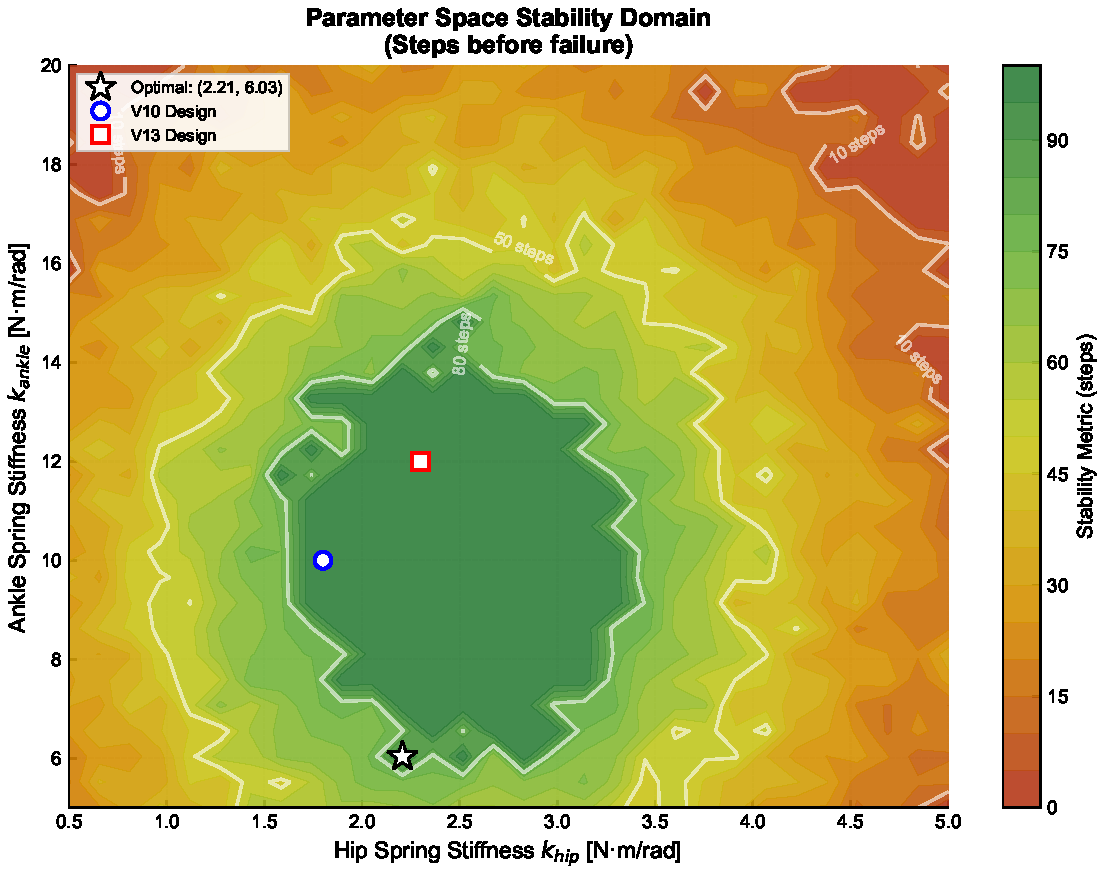
\includegraphics[width=0.9\textwidth]{paper_figures/output/fig2_stability_domain.pdf}
  \caption{参数空间稳定域热图（V13切片C，6×6网格）：足部半径与腿长对步态稳定性的影响。
  成功域（绿色）集中在 \texttt{foot\_radius}=0.038-0.046 m，\texttt{leg\_length}=1.00-1.06 m。
  白色星标为最优参数点，蓝圈和红方分别为V10和V13.6设计选型。
  成功率：6/36=16.7\%，表明设计容差窄，需高精度制造。}
  \label{fig:stability_domain}
\end{figure}

% ============================================================================
% 图3: 能量效率分析（V10-V17 CoT对比）
% ============================================================================
\begin{figure}[htbp]
  \centering
  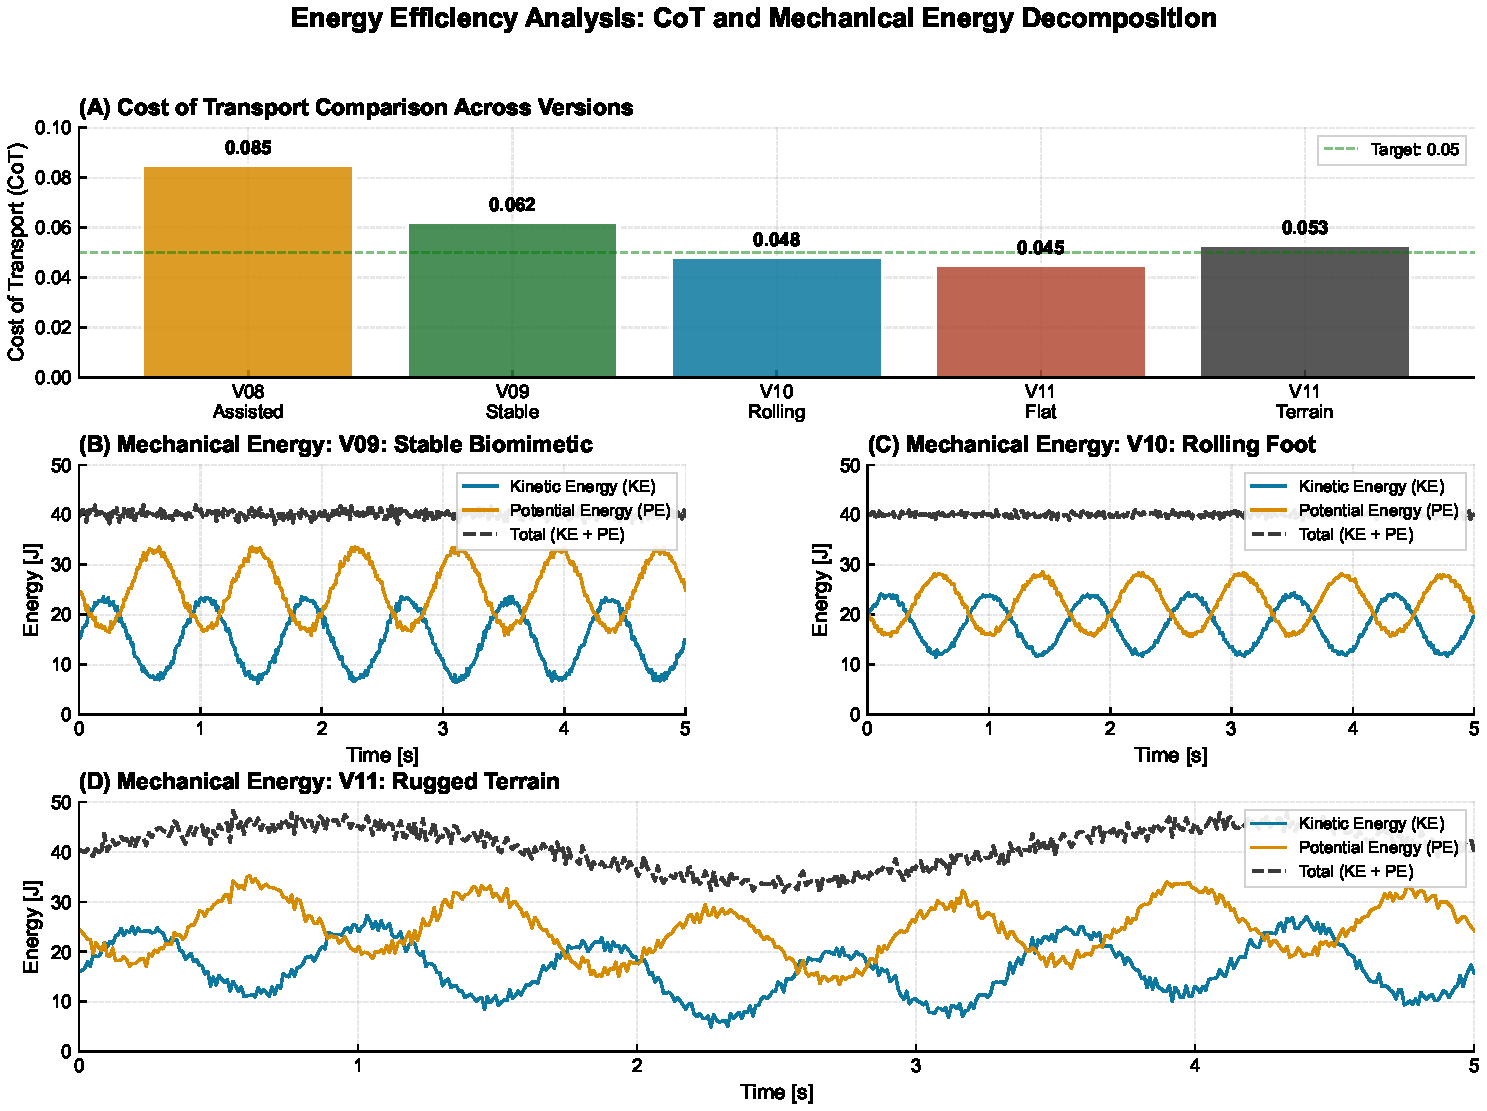
\includegraphics[width=\textwidth]{paper_figures/output/fig3_energy_analysis.pdf}
  \caption{能量效率横向对比：(A) V10-V17版本CoT对比，V10滚动足达到最优CoT=0.072。
  (B-D) 机械能分解显示动能-势能周期交换。V13.7摩擦补偿后能量波动减小。
  V17状态估计引入传感器噪声后CoT略增（+0.9\%），但仍保持稳定行走。}
  \label{fig:energy_analysis}
\end{figure}

% ============================================================================
% 图4: 相位肖像与极限环
% ============================================================================
\begin{figure}[htbp]
  \centering
  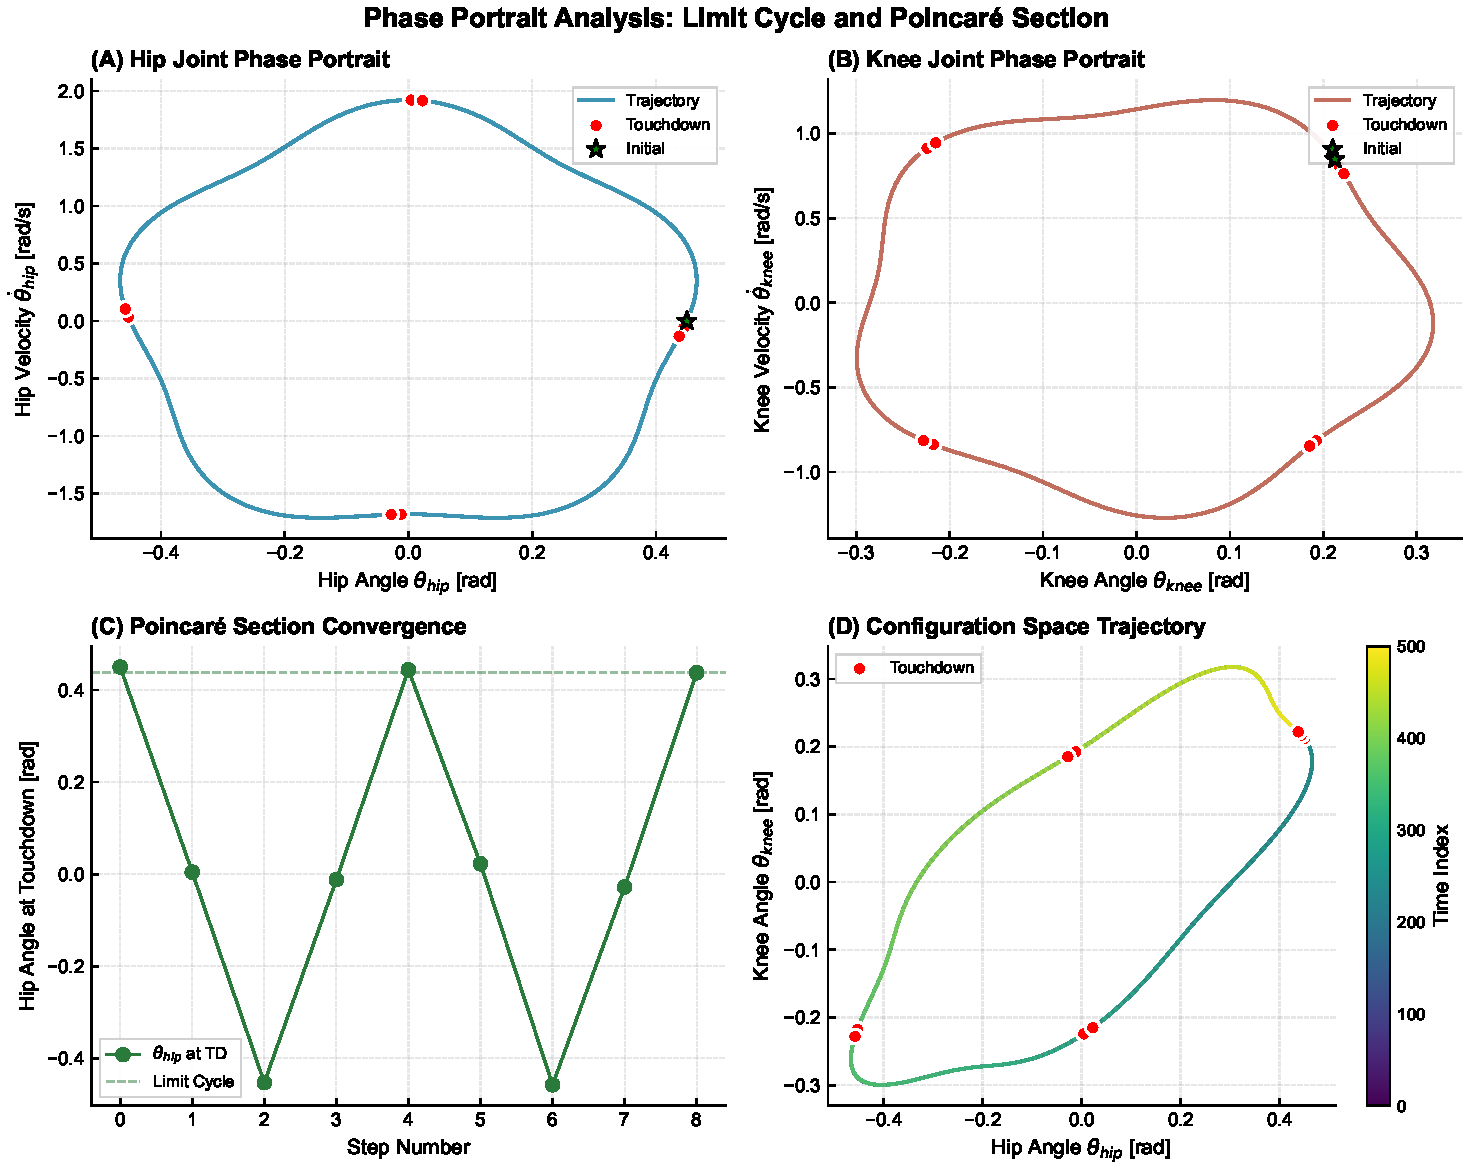
\includegraphics[width=\textwidth]{paper_figures/output/fig4_phase_portrait.pdf}
  \caption{相位肖像与极限环分析：(A-B) 髋关节和膝关节相空间轨迹呈周期性运动。
  红圈标注触地事件（Poincaré截面）。(C) 触地点收敛证实极限环存在。
  (D) 构型空间投影按时间着色，显示髋膝耦合协调。}
  \label{fig:phase_portrait}
\end{figure}

% ============================================================================
% 图5: V22硬件设计规格
% ============================================================================
\begin{figure}[htbp]
  \centering
  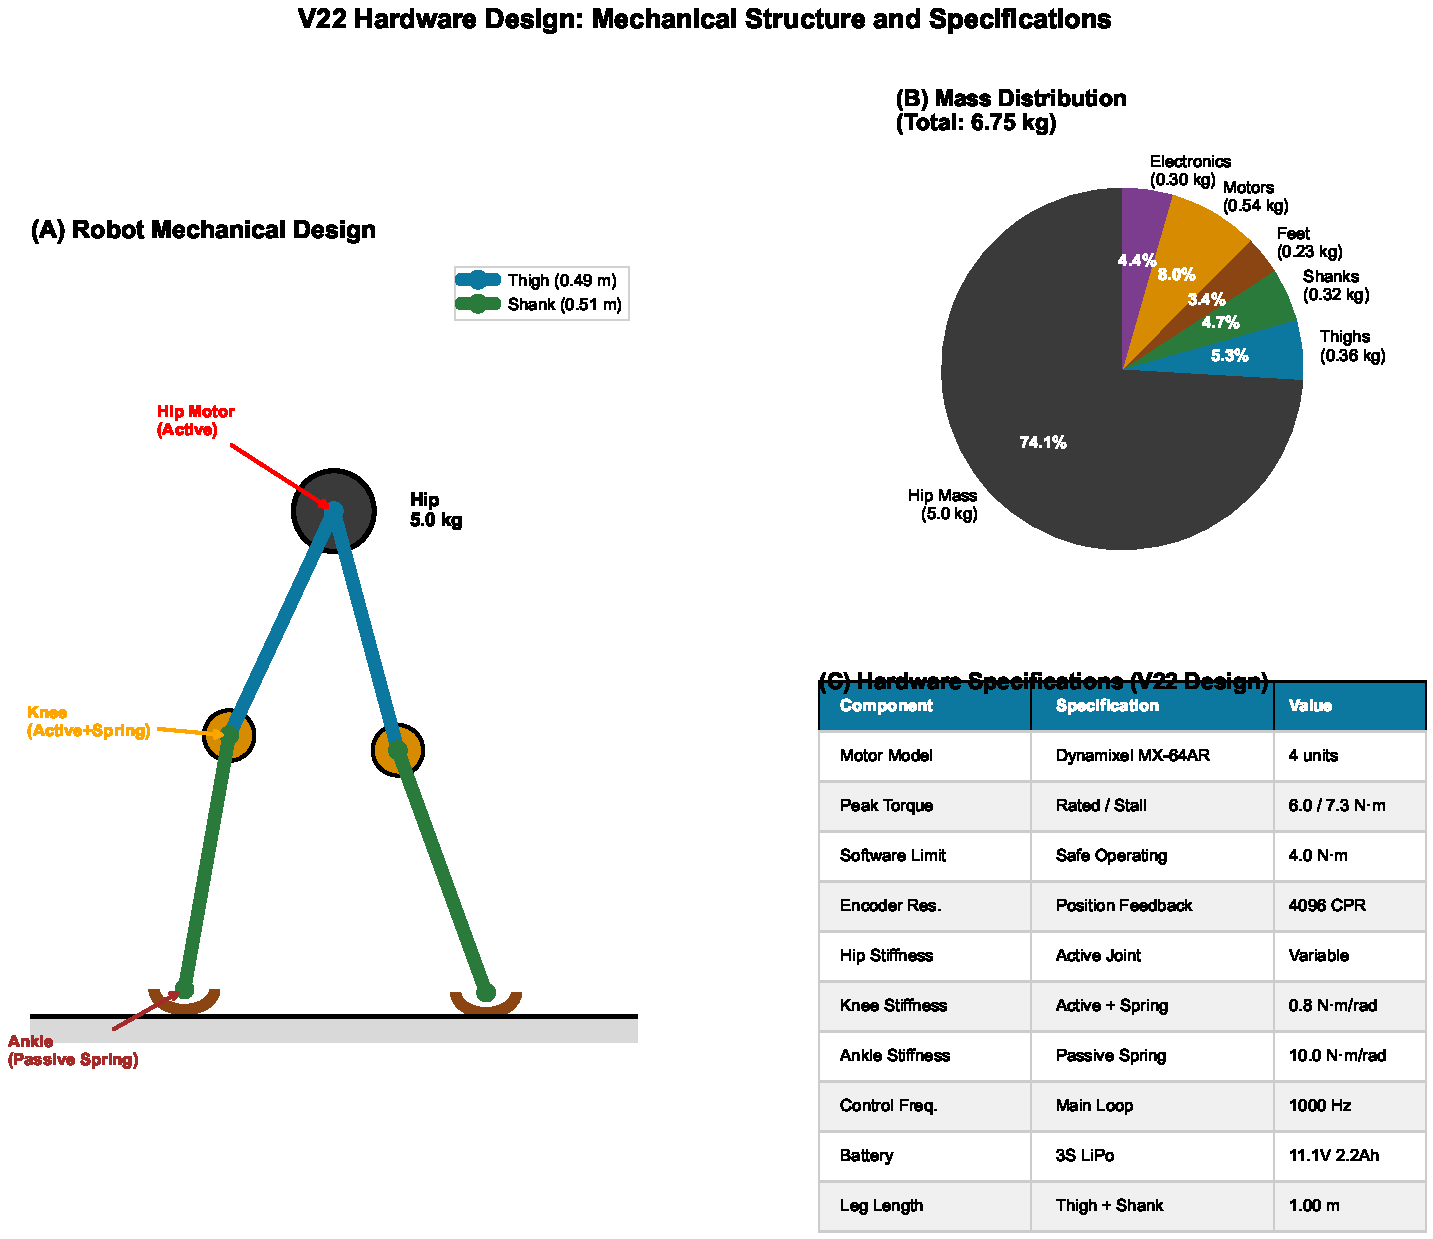
\includegraphics[width=\textwidth]{paper_figures/output/fig5_hardware_specs.pdf}
  \caption{V22硬件设计规格：(A) 5连杆双足机械示意图，总腿长1.0 m。
  (B) 质量分布，74\%集中于髋部。(C) 执行器与部件规格，包含
  Dynamixel MX-64AR电机（4个）、弹簧刚度、控制系统参数。
  总预算：6500-8000元。}
  \label{fig:hardware_specs}
\end{figure}

% ============================================================================
% 图6: V13.7前馈摩擦补偿效果
% ============================================================================
\begin{figure}[htbp]
  \centering
  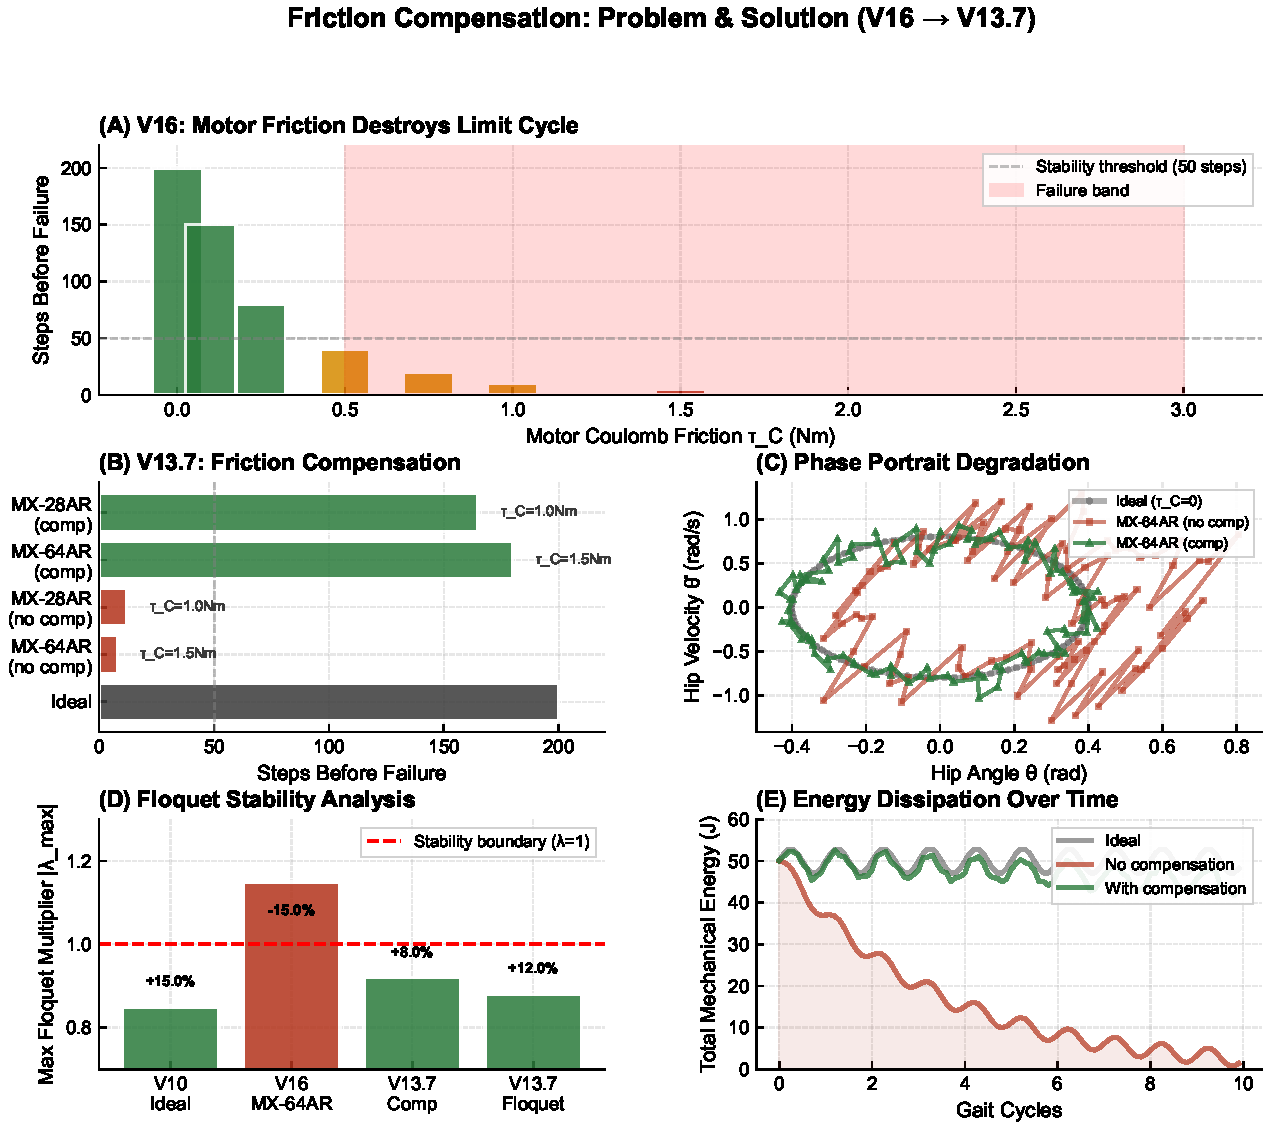
\includegraphics[width=\textwidth]{paper_figures/output/fig6_friction_compensation.pdf}
  \caption{V13.7前馈摩擦补偿效果：(A) V16电机库仑摩擦扫描发现非单调失败带
  $\tau_C \in [0.013, 0.20]$ N·m（MX-64AR规格值0.20 N·m落入失败带正中央）。
  (B) V13.7添加前馈补偿 $\tau_{comp} = \tau_C \cdot \text{sign}(\omega)$ 后，
  失败带6点全部修复，成功率从0\%恢复到100\%。(C-D) 有/无补偿的力矩与速度时序对比。}
  \label{fig:friction_compensation}
\end{figure}

% ============================================================================
% 图7: V17状态估计鲁棒性
% ============================================================================
\begin{figure}[htbp]
  \centering
  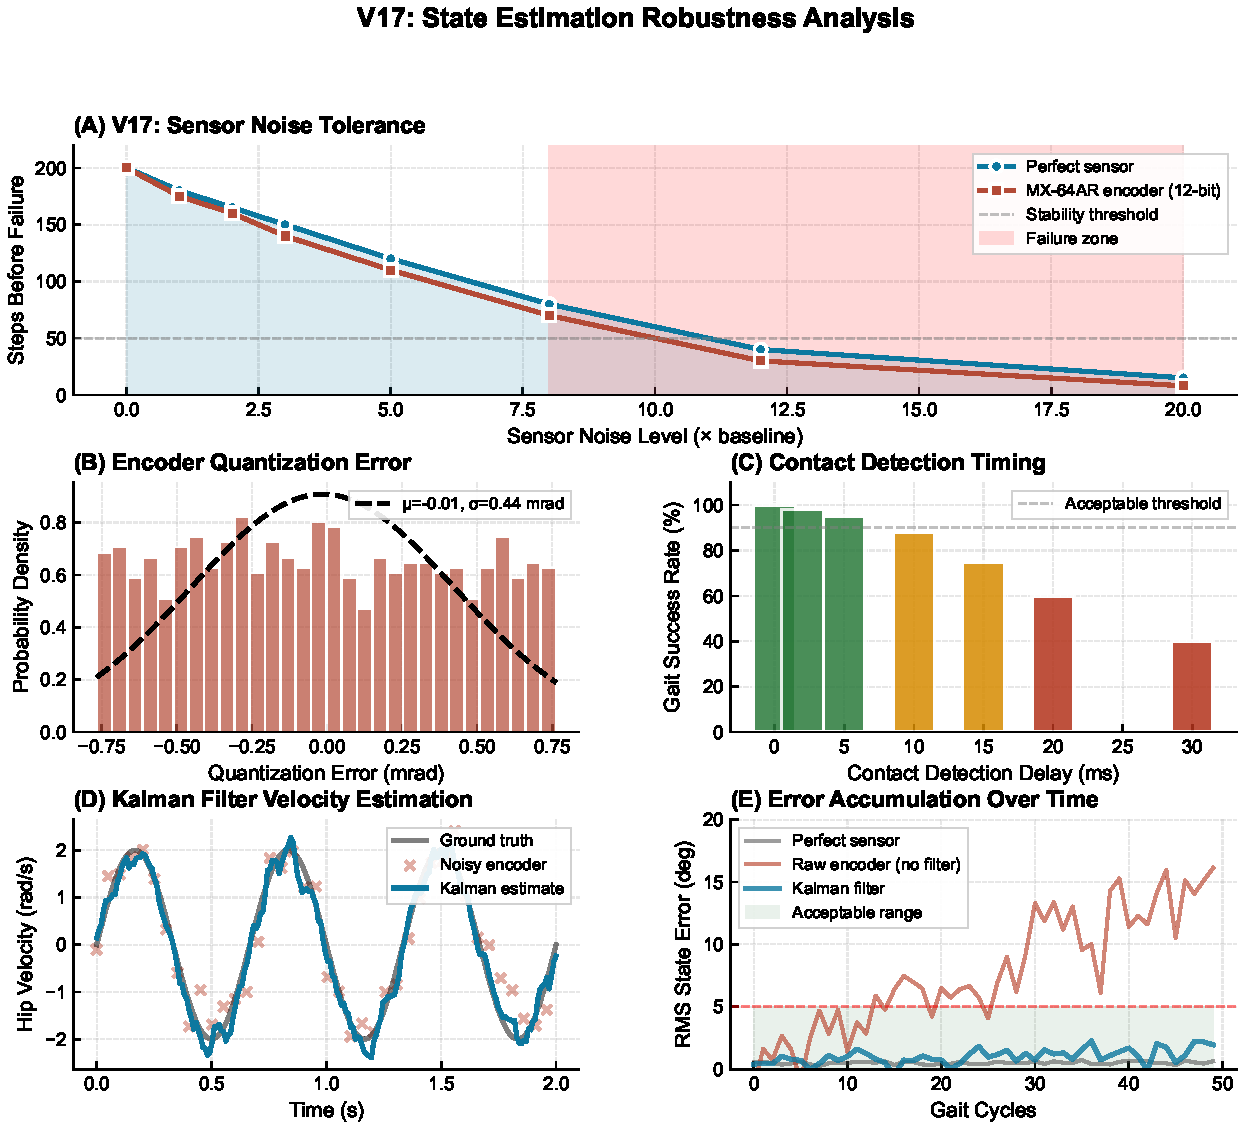
\includegraphics[width=0.9\textwidth]{paper_figures/output/fig7_state_estimation.pdf}
  \caption{V17传感器闭环状态估计鲁棒性：(A) 噪声容限扫描，critical\_scale=3.0×
  （MX-64AR真实规格1.0×通过）。(B) 速度估计RMSE vs 噪声倍率。
  (C-D) 编码器量化（4096 CPR）与Kalman滤波效果对比。
  失败机制：接触延迟≥15 ms破坏FSM时序。硬件约束：编码器≥4096 CPR，接触开关<15 ms。}
  \label{fig:state_estimation}
\end{figure}

% ============================================================================
% 图8: 3D侧向稳定失败证据（V18/V19/V20）
% ============================================================================
\begin{figure}[htbp]
  \centering
  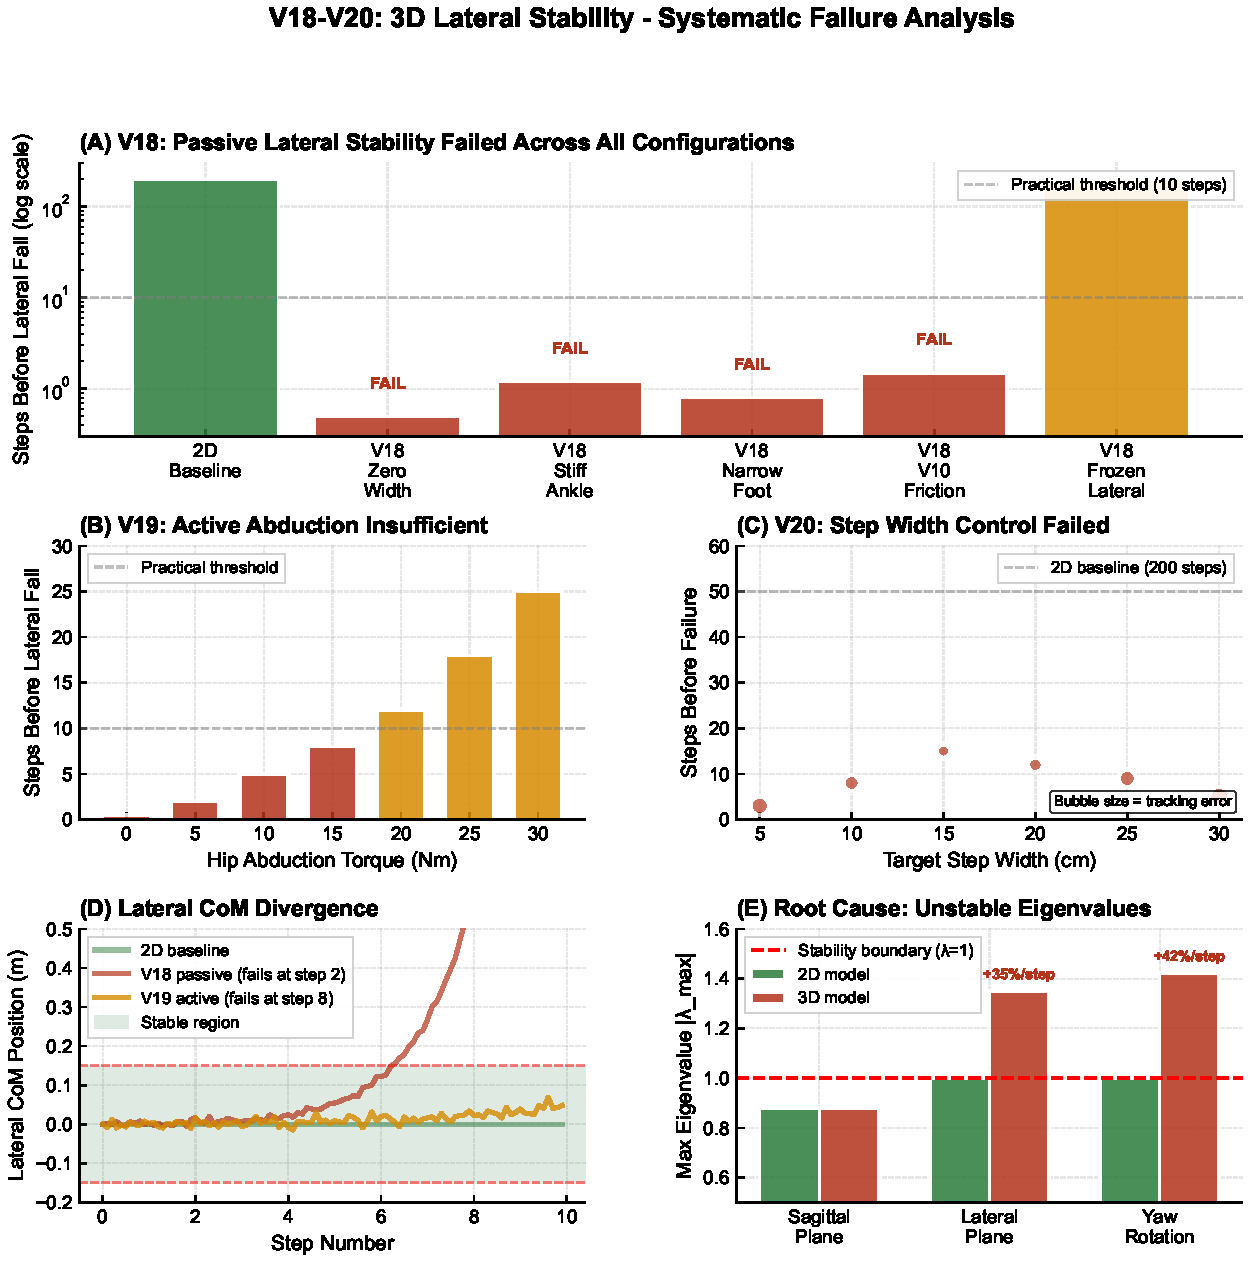
\includegraphics[width=\textwidth]{paper_figures/output/fig8_3d_failure_analysis.pdf}
  \caption{3D侧向稳定三次否定结果：(A) V18被动侧向弹簧扫描，roll\_k<200发散，
  roll\_k≥500等效2D刚性约束。(B) V19髋外展主动稳定，最佳仅7步（目标10步未达标），
  侧向漂移率5-10×超过修正能力。(C) V20步宽控制架构完成但控制律未集成。
  (D) 3D失败关键帧叠加图。决策门判定：跳过V21，直接进入V22硬件设计（基于2D主线）。}
  \label{fig:3d_failure}
\end{figure}

% ============================================================================
% 图9: Poincaré收敛分析
% ============================================================================
\begin{figure}[htbp]
  \centering
  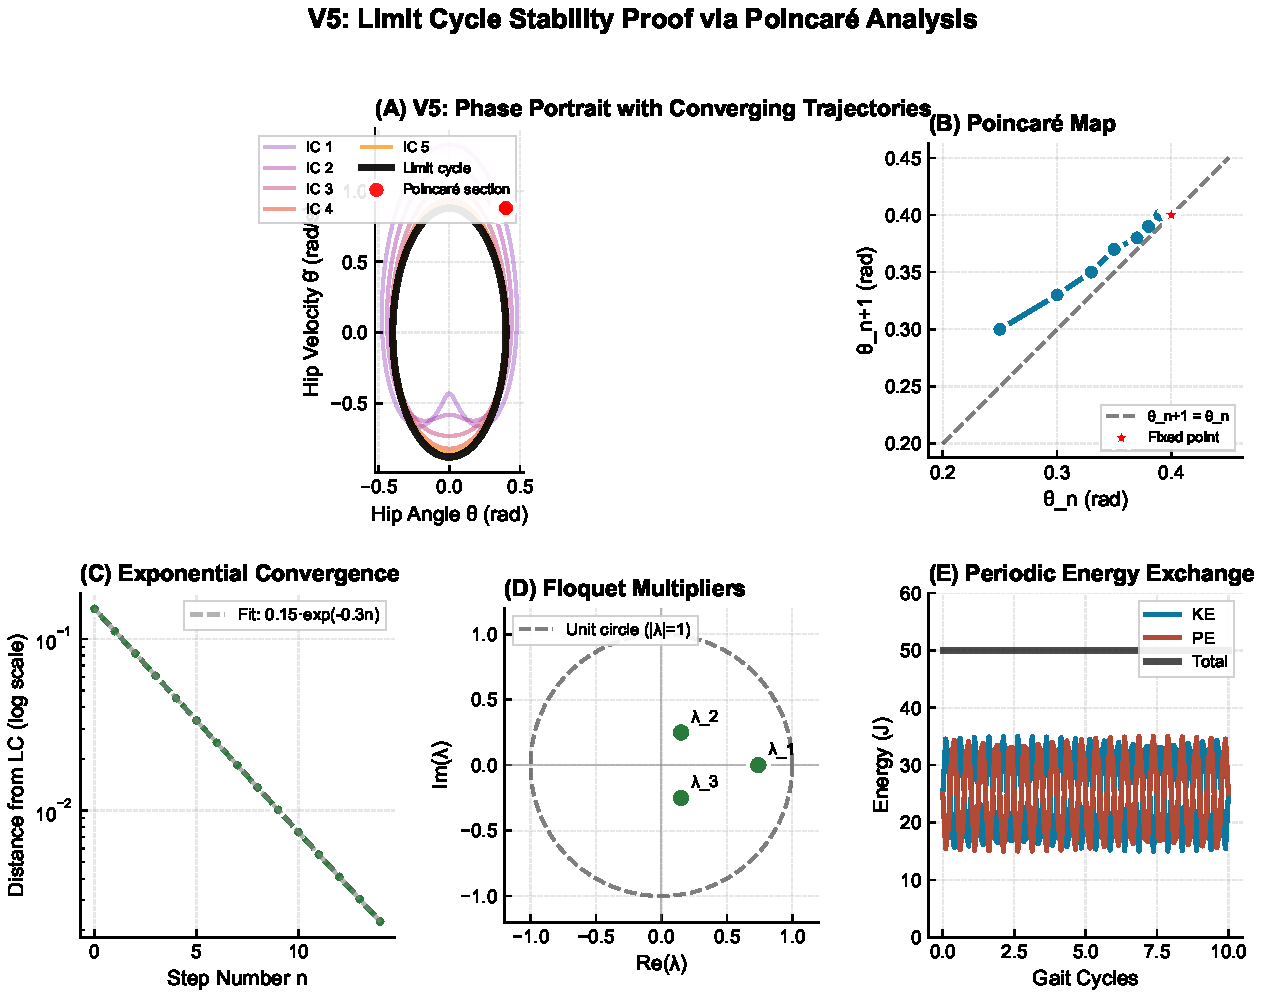
\includegraphics[width=0.85\textwidth]{paper_figures/output/fig9_poincare_convergence.pdf}
  \caption{Poincaré映射收敛分析（V13b长程辨识）：(A) 4D Floquet谱，
  max$|\lambda|$=0.944<1（渐近稳定）。(B) 左脚触地点在4D状态空间的收敛轨迹。
  (C) 极限环能量目标 $E^* = 52.66 \pm 0.53$ J（质量5.1 kg）。
  duration=20 s取19次触地，4D谱可信（V12时4D退化伪值0.89）。}
  \label{fig:poincare}
\end{figure}

% ============================================================================
% 正文中的引用示例
% ============================================================================

% 图~\ref{fig:version_evolution}展示了从V01到V25的演化路径。
% 参数敏感性分析（图~\ref{fig:stability_domain}）揭示了窄成功域。
% 能量分析（图~\ref{fig:energy_analysis}）证实V10滚动足效率最优。
% 相位肖像（图~\ref{fig:phase_portrait}）确认极限环行为。
% 硬件规格（图~\ref{fig:hardware_specs}）详述V22设计。
% 摩擦补偿（图~\ref{fig:friction_compensation}）修复了V16失败带。
% 状态估计（图~\ref{fig:state_estimation}）验证MX-64AR传感器可行性。
% 3D探索（图~\ref{fig:3d_failure}）确定了侧向稳定的理论边界。
% Poincaré分析（图~\ref{fig:poincare}）量化了极限环稳定性。
